\section{Pixelar}
Este filtro consiste en tomar bloques de 2x2 píxeles y asignarles a estos el promedio del bloque. De esta manera se disminuye la cálidad de la imágen.
\subsection{Código C}
	El código de C consiste en recorrer la imagen de a dos filas y dos columnas por iteración. En cada iteración se calcula el promedio de los canales de los píxeles.
	A continuación adjuntamos el pseudocódigo.

\begin{algorithm}[h!]
\caption{Promedio}
\begin{algorithmic}
  \Function{promedio}{$a :~unsigned~ char, ~b:~ unsigned ~char, ~c: ~unsigned~ char, ~d: ~unsigned~ char$}  $\to \texttt{float}$
	\State $float~ af \gets a$
	\State $float~ bf \gets b$
	\State $float~ cf \gets c$
	\State $float~ df \gets d$
	\State \Return $(af/4+bf/4+cf/4+df/4)$
	
\EndFunction
\end{algorithmic} 
\end{algorithm}	
	
	\begin{algorithm}[h!]
\caption{Pixelar}
\begin{algorithmic}
  \Function{pixelar}{src: *unsigned char, dst: *unsigned char, cols: int, filas: int, srcRowSize: int, dstRowSize: int}
	\State $unsigned~ char~ (*srcMatrix)[srcRowSize] = (unsigned~ char (*)[srcRowSize])~ src$
	\State $unsigned~ char~ (*dstMatrix)[dstRowSize] = (unsigned~ char (*)[dstRowSize])~ dst$
	
	\For{$f \gets 0~..~filas-1; f+=2$}
		\For{$c \gets 0~..~cols-1; c+=2$}
			\State $bgra_t* p_s1 \gets (bgra_t*)$ \& $srcMatrix[f][c * 4]$
			\State $bgra_t *p_d1 \gets (bgra_t*)$ \&$dstMatrix[f][c * 4]$
			
			\State $bgra_t* p_s2 \gets (bgra_t*)$ \& $srcMatrix[f+1][c * 4]$
			\State $bgra_t *p_d2 \gets (bgra_t*)$ \&$dstMatrix[f+1][c * 4]$
			
			\State $bgra_t* p_s3 \gets (bgra_t*)$ \& $srcMatrix[f+1][(c+1) * 4]$
			\State $bgra_t *p_d3 \gets (bgra_t*)$ \&$dstMatrix[f+1][(c+1) * 4]$
			
			\State $bgra_t* p_s4 \gets (bgra_t*)$ \& $srcMatrix[f][(c+1) * 4]$
			\State $bgra_t *p_d4 \gets (bgra_t*)$ \&$dstMatrix[f][(c+1) * 4]$
			
			\State k $\gets$ 0.5
			
			\State b $\gets$ \Call{promedio}{$p_s \rightarrow b, p_s2 \rightarrow b, p_s3 \rightarrow b, p_s4 \rightarrow b$}
			\State g $\gets$ \Call{promedio}{$p_s \rightarrow g, p_s2 \rightarrow g,p_s3 \rightarrow g, p_s4 \rightarrow g$}
			\State r $\gets$ \Call{promedio}{$p_s \rightarrow r, p_s2 \rightarrow r, p_s3 \rightarrow r, p_s4 \rightarrow r$}
			\State a $\gets$ \Call{promedio}{$p_s \rightarrow a, p_s2 \rightarrow a, p_s3 \rightarrow a, p_s4 \rightarrow a$}
				
			\For{$i \gets 1~..~4$}
				\State ($p_di \rightarrow$b) $\gets$ b
				\State ($p_di \rightarrow$g) $\gets$ g
				\State ($p_di \rightarrow$r) $\gets$ r
				\State ($p_di \rightarrow$ a) $\gets$ a
			\EndFor
		\EndFor
	\EndFor
\EndFunction

\end{algorithmic} 
\end{algorithm}
\subsection{Código ASM}
El codigo en ASM consiste en una union de cilos, uno exterior para iterar sobre las filas y otro interior para iterar sobre los elemntos de la misma (columnas). Lo que hace este codigo es en cada iteracion, lee de memoria dos veces, empezando en la misma columna pero de dos filas diferentes. De esta forma levanta como una matriz de 8 elementos (4x2). Lo que se puede obtener de esta informacion va a servir para sobre escribir 8 pixeles. \\ El ciclo luego procede en exteneder los signos de cada byte, luego guardar la sumatoria de los elementos {1,2,6,7} (mirandolo como una matriz de 4x2), y la sumatoria de {4,5,8,9} en dos registros aparte, calcular el promedio de esto, osea dividirlos por cuatro. Y luego a esta informacion la volvemos a agrupar juntas en un mismo registro que se veria de esta manera :

\par{\textbf{XMM:}}
\xmmb{$Pp1_a$}{$Pp1_r$}{$Pp1_g$}{$Pp1_b$}{$Pp1_a$}{$Pp1_r$}{$Pp1_g$}{$Pp1_b$}{$Pp2_a$}{$Pp2_r$}{$Pp2_g$}{$Pp2_b$}{$Pp2_a$}{$Pp2_r$}{$Pp2_e$}{$Pp2_b$}
\par {Pp1 : promedio pixeles {1,2,6,7}. Pp2 : promedio pixeles {4,5,8,9}}
	
	
.\\ Y finalmente a este registro lo escribimos en la imagen destino, en los lugar de los cual levantamos en la imagen src. \\ Por ultimo movemos los current en columnas 4 pixeles que es la cantidad sobre esa fila q procesamos en cada iteracion. Y si terminamos de procesar la fila, nos movemos dos filas, ya que vamos procesando dos juntas a la vez.
	
\subsection{Experimentación 1}
\subsubsection{Idea}	
	Comparamos la eficacia del código en ASM contra C y C optimizado.
	
\subsubsection{Resultados}
	\begin{figure}[h!]
	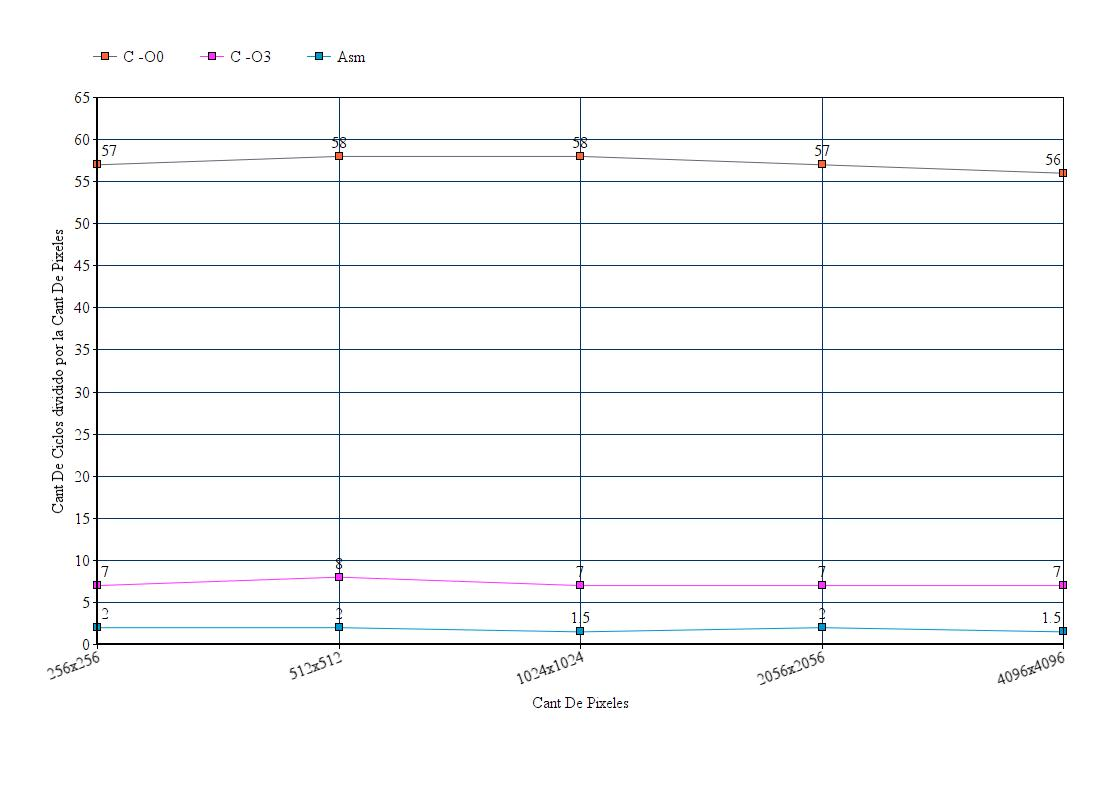
\includegraphics[width = 15 cm, height = 10 cm]{imagenes/pixeAsmC.png}
	\caption[center]{Comparacion (ciclos Totales) / (cant De pixeles) - diferentes Implementaciones de C y Asm}
\end{figure}

\subsection{Experimentacion 2}
\subsubsection{Idea}
Comparamos la eficacia entre utilizar instrucciones como shift, para dividir los pixeles, contra las instrucciones para dividir floats, que implican ademas tener que hacer un traspaso de formato.

\subsubsection{Hipotesis}
Nuestra idea es que va a ser mucho mas optimo el codigo donde utilizamos las intrucciones de shift para dividir los nunmeros, porque son operaiones basicas que se encarga el registro de hacerlas, en cambio el pasar a float, dividir luego y volver  a pasar a float, son todas operaciones sin implementacion primitiva, osea por esto nos referimos a que estan compuestas de varias otras instrucciones y hace que la ejecucion de cada una demore varios ciclos mas que un simple shift.

\subsubsection{Resultados}
	\begin{figure}[!h]
	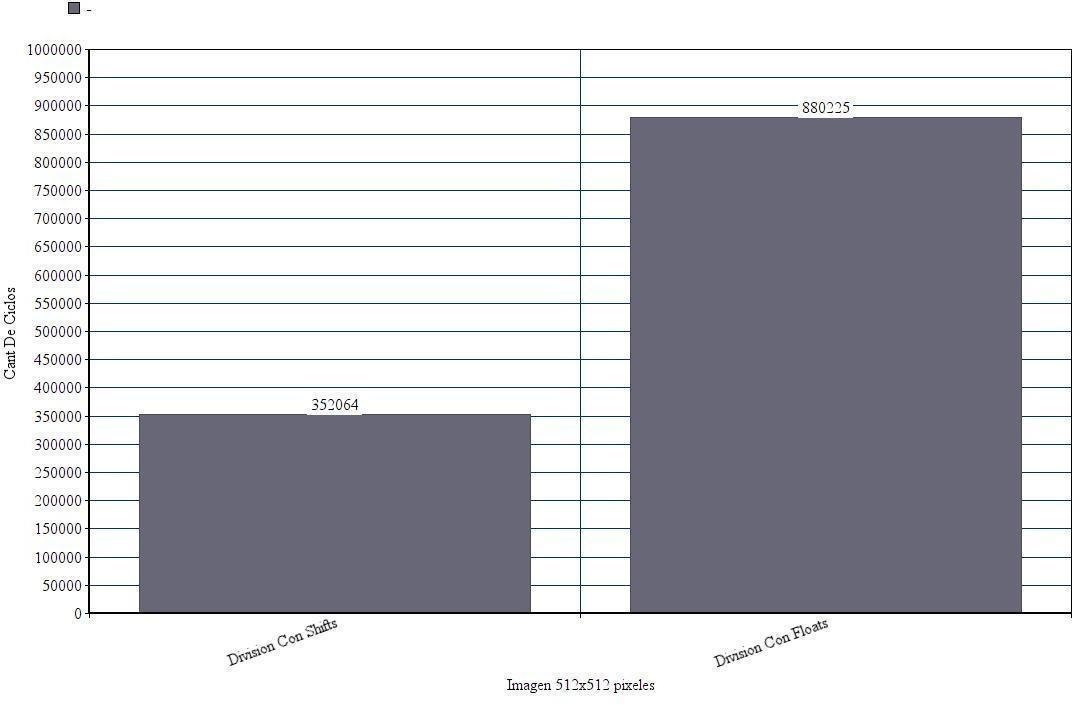
\includegraphics[width = 15 cm, height = 10 cm]{imagenes/Div_pixelar.jpg}
	\end{figure}
	
\subsubsection{Conclucion}
	Definitivamente el codigo en el cula dividimos con shifts fue mucho mas optimo, denuevo por lo que explicamos en la hipotesis.